\documentclass[11pt]{article}
\usepackage{amsmath,amssymb,amsfonts,amsbsy}
\usepackage{float}
%\usepackage{fancybox}
\usepackage{fancyhdr}
\usepackage{booktabs}
\usepackage[table]{xcolor}
\usepackage{graphicx}
\usepackage{soul,soulutf8}
\usepackage{url,color}
\usepackage{fullpage}
\usepackage{bm}
\usepackage{listings}
\RequirePackage{listings}
\RequirePackage{xcolor}
\definecolor{dkgreen}{rgb}{0,0.6,0}
\definecolor{gray}{rgb}{0.5,0.5,0.5}
\definecolor{mauve}{rgb}{0.58,0,0.82}
\lstset{
  frame=tb,
  aboveskip=3mm,
  belowskip=3mm,
  showstringspaces=false,
  columns=flexible,
  framerule=1pt,
  rulecolor=\color{gray!35},
  backgroundcolor=\color{gray!5},
  basicstyle={\small\ttfamily},
  numbers=none,
  numberstyle=\tiny\color{gray},
  keywordstyle=\color{blue},
  commentstyle=\color{dkgreen},
  stringstyle=\color{mauve},
  breaklines=true,
  breakatwhitespace=true,
  tabsize=3,
}

\baselineskip=15pt
\pagestyle{plain}   %with page numbers
%\pagestyle{empty} %without page numbers

\renewcommand{\baselinestretch}{1.25}
\newcommand{\R}{\mathbb{R}}
\newcommand{\cX}{\mathcal{X}}
%\newcommand{\tr}{\mathrm{tr}}
\renewcommand{\st}{\mathrm{s.t.}}

\begin{document}

\begin{center}
{\large CIE6010/MDS6118 (F2018)}
{\Large\bf Assignment 1}\\[.2in]
Name (Chinese and English): \underline{\hspace*{2in}}\\[.1in]
Course Number (taken by you): \underline{\hspace{2in}}
\end{center}
\medskip


A general optimization problem is
\begin{eqnarray*}
\min && f(x) \\
\st && x \in \cX
\end{eqnarray*}

{\bf Exercise 1.1.8}
We set the coordinate of $p$ and $q$ on the plane to be:
\[
\begin{array}{ll}
p=\begin{pmatrix}
p_1\\p_2
\end{pmatrix}
&
q=\begin{pmatrix}
q_1\\q_2
\end{pmatrix}
\end{array}
\]
Let $x$ denote the horizontal coordinate of the intersection between the ray of light and the horizontal axis.



\begin{itemize}
\item The objective function is the travel time of the light, i.e.,
\[
f(x) = \frac{1}{v}\sqrt{(p_1-x)^2+p_2^2}+\frac{1}{w}\sqrt{(q_1-x)^2+q_2^2}
\]

\item The feasibility set is
\[
\cX = [\min\{p_1,q_1\},\max\{p_1,q_1\}]
\]

\item When $v=w$, the solution is
\[
x = \frac{|q_2|}{|p_2|+|q_2|}p_1+\frac{|p_2|}{|p_2|+|q_2|}q_1
\]
This is because by settign $f'(x)=0$, we derive:
\[
\frac{1}{v}\frac{x-p_1}{2\sqrt{(x-p_1)^2+p_2^2}}+\frac{1}{w}\frac{x-q_1}{2\sqrt{(x-q_1)^2+q_2^2}}=0
\]
Or equivalently,
\[
(x-p_1)^2[(x-p_1)^2+p_2^2]=(x-q_1)^2[(x-q_1)^2+q_2^2]
\implies (x-p_1)|q_2| = (q_1-x)|p_2|
\]
After simplification, the optimal solution is obtained:
\[
x=\frac{|q_2|}{|p_2|+|q_2|}p_1+\frac{|p_2|}{|p_2|+|q_2|}q_1
\]
\end{itemize}



\clearpage
\section*{The screen printout from my run}
\begin{figure}[H]
\centering
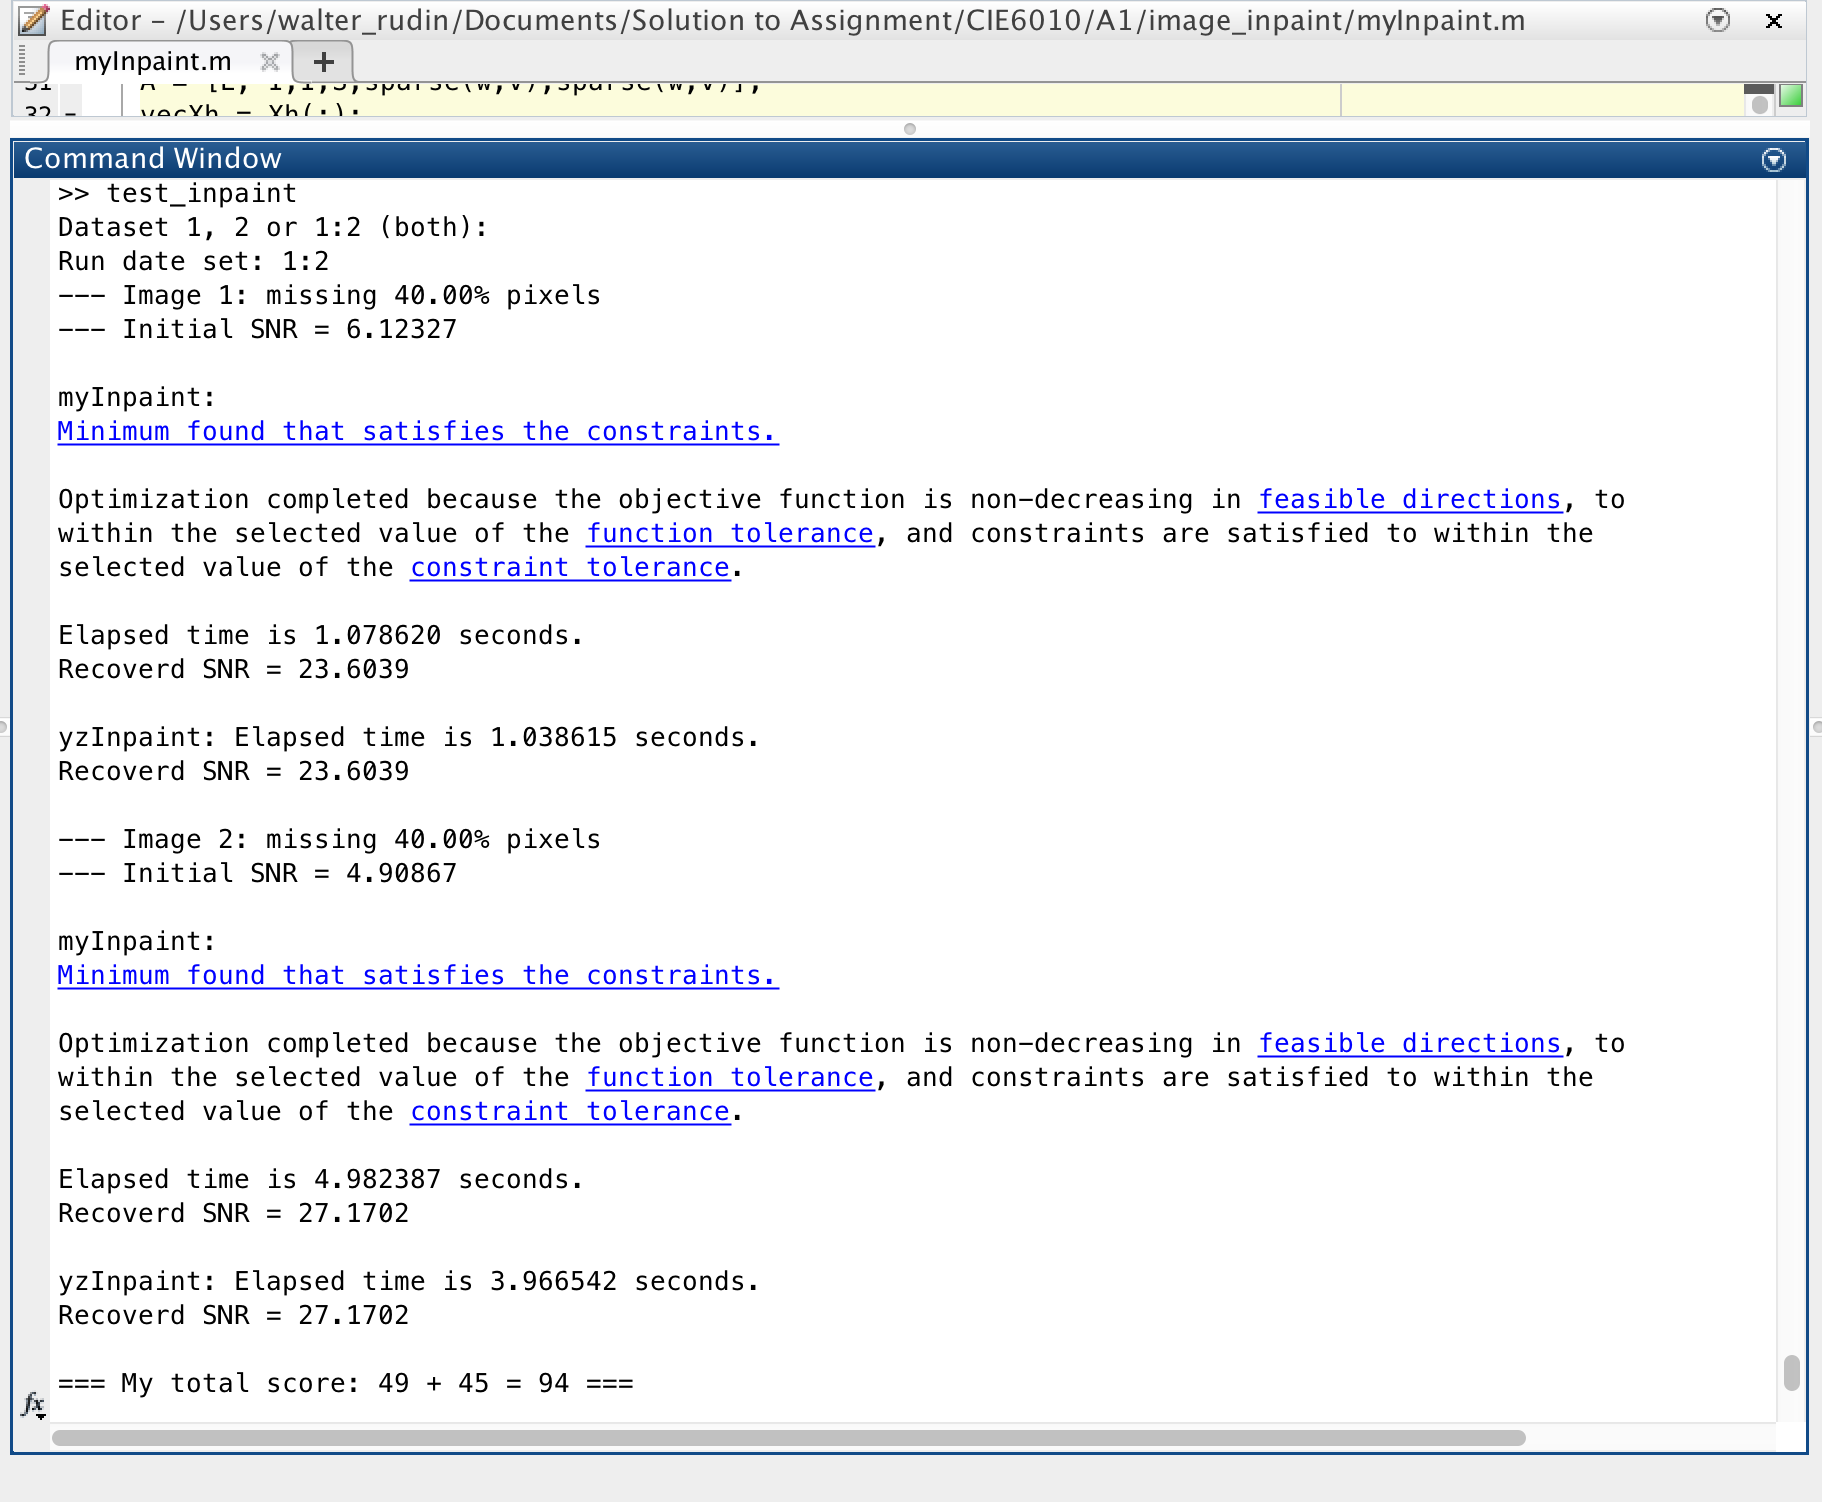
\includegraphics[height=12cm]{Print_out}
\caption{Printout from Run}
\label{Printout from Run}
\end{figure}
\clearpage
\section*{Generated Figures from my code}
\begin{figure}[H]
\centering
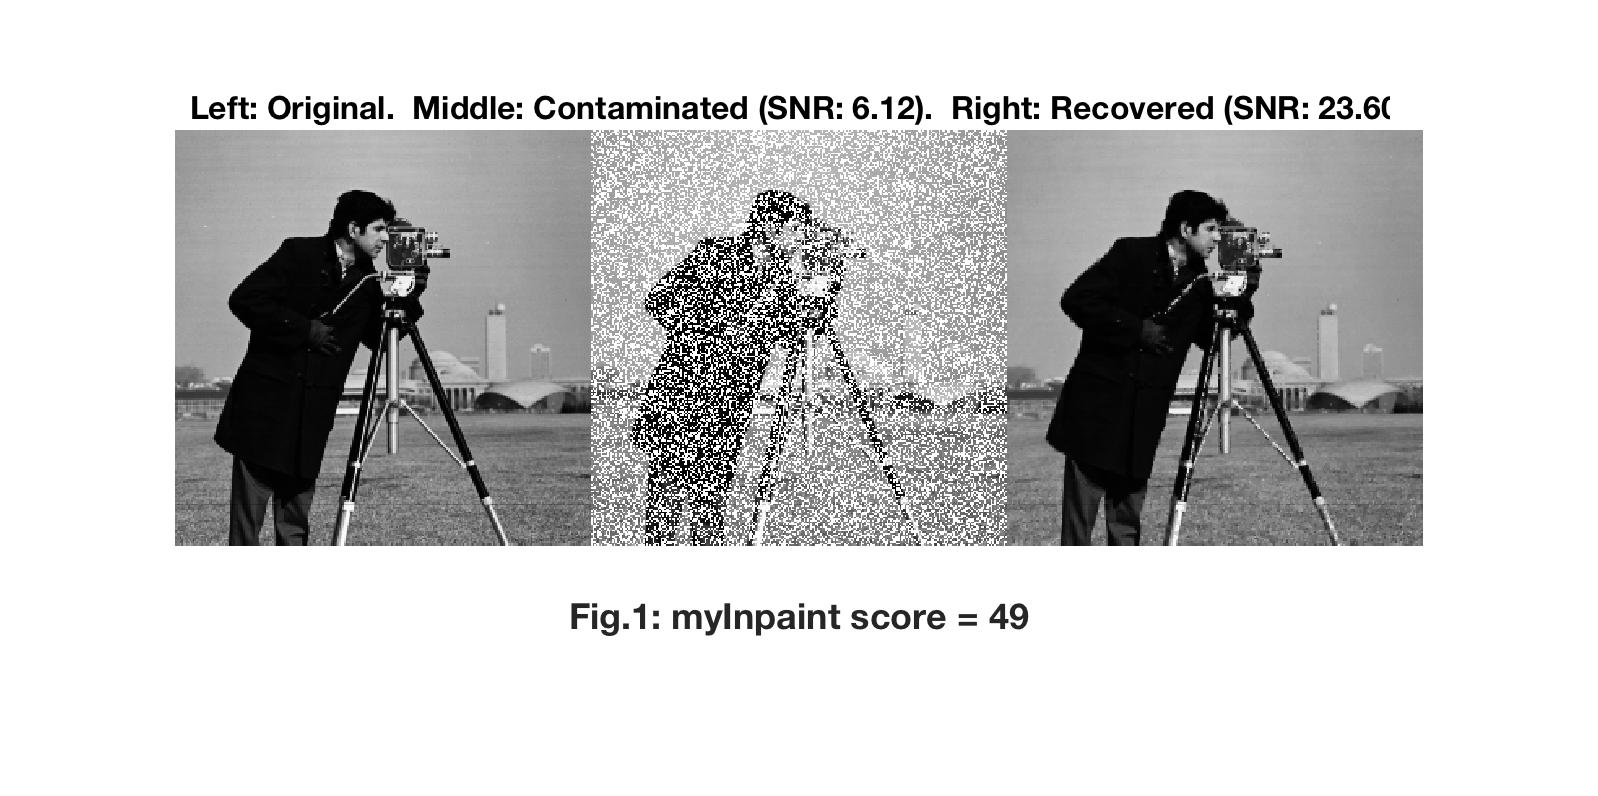
\includegraphics[width=14cm]{Fig_1}
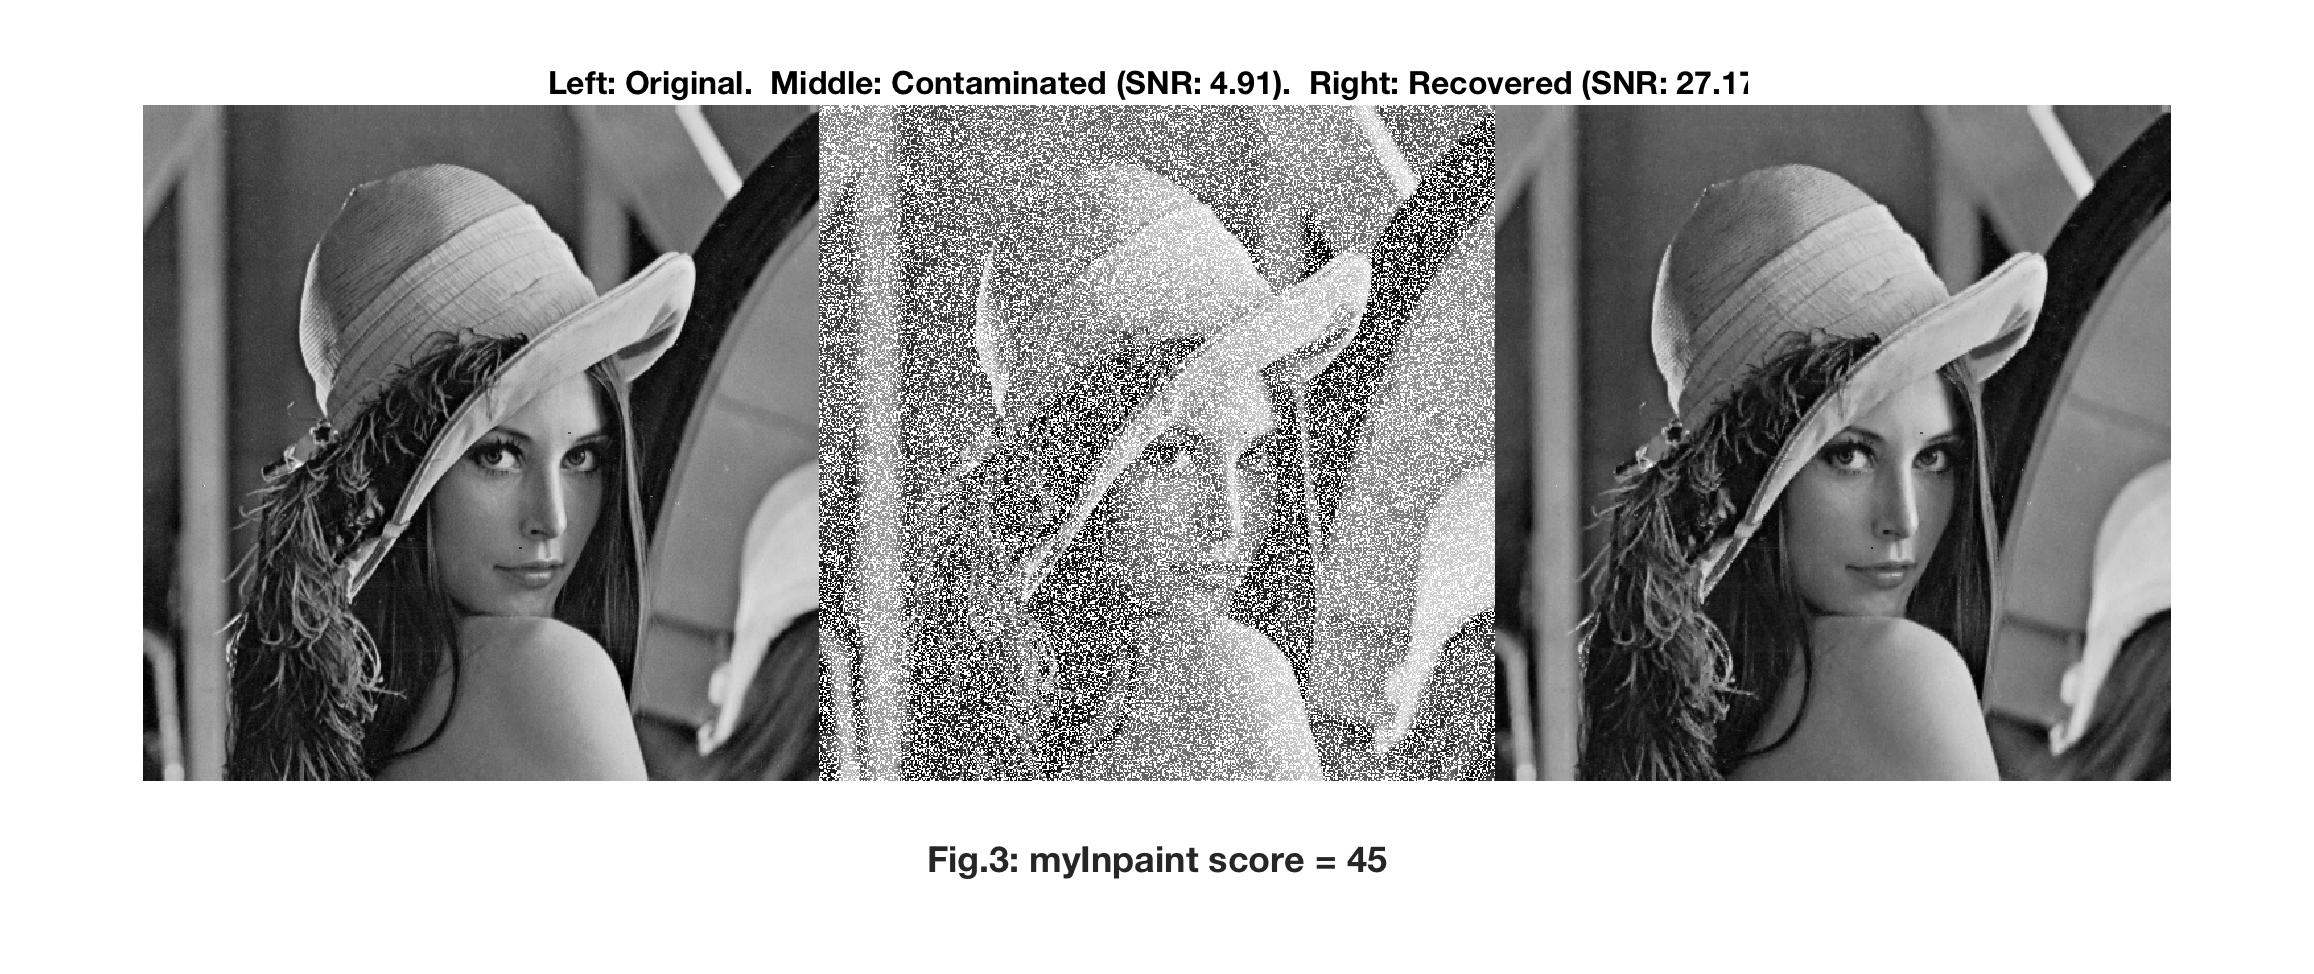
\includegraphics[width=14cm]{Fig_3}
\caption{Output of my code}
\end{figure}




\clearpage
\section*{Summary of Matlab Project}
\begin{itemize}
\item
This project is to de-noise an image with a large number of missing pixels at random locations by solving a linear programming problem.
\item
The idea is to fill in missing pixels such that the output image has a small total variation. The details of the procedure are given as follows:
\item
Given the available matrix $\hat X\in\mathbb{R}^{n\times n}$ and $\Omega\in\mathbb{R}^{m\times 1}$, use command $\textsf{length}$ to find $m$ and $n$.
\item
To find $E\in\mathbb{R}^{}$, we first create $D$ by using $\textsf{speye}$ and adding $-1$s on the first above diagonal; then $E$ is computed as $\textsf{E = [kron(I,D);[kron[D,I]];}$ with $I$ to be identity matrix with size $n$.
\item
$S$ is a sub-matrix of identity matrix of size $n^2$, consisting of the rows whose indices are in $\Omega$. We use the command given below to compute $S$:
\begin{verbatim}
i = 1:m;		j = Omega;	v = 1 * ones(m,1);  S = sparse(i,j,v,m,n^2)
\end{verbatim}
\item
Then we compute $\bm A$ by using the command $\textsf{[E,-I,I;S,sparse(w,v),sparse(w,v)];}$, where $\textsf{I}$ are all identity matrices of size $n(n-1)$.
\item
$f$ is a vector of size $(m+2n^2-n)$, with the first $m$th entries to be zero, the remaining entries to be one. $\bm b$ is a vector of size $n^2-n+m$, with the first $n^-n$ entries to be zero, the last $m$ entries to be the available pixel values with indices in $\Omega$.
\item
Call the MATLAB command $\textsf{z = linprog(f,[],[],A,b,LB,UB,options)}$ to get optimal solution $\bm z$, where the $\textbf{LB}$ is a vector consisting zero entries; $\textsf{UB}$ is a vector consisting $\textsf{Inf}$ entries; options are the \textit{interior-point} algorithm.
\item
$\bm x$ is the first $n^2$ entries of $\bm z$, and then we reshape it into $n\times n$ matrix to get recovered image $X$ for output.

\end{itemize}
\clearpage
\section*{A Copy of my Code myInpaint.m.}
\begin{lstlisting}[language=matlab]
function [ X ] = myInpaint( Xh, Omega )
%      Usage:
%      Input:
%         Xh: the available matrix, with size n*n
%      Omega: the available pixel set Omega, with size m
%     Output:
%          X: the recovered graph

%% Figure Out relevant sizes
n = length(Xh);
m = length(Omega);

%% Construct the E matrix and the S matrix
I = speye(n,n);
% Generate vectors of subscripts and corresponding values of D
i = 1:n-1;
%j = 2:n;
v = -1 * ones(n-1,1);
D = sparse(i,i+1,v,n-1,n) + speye(n-1,n);
E = [kron(I,D);kron(D,I)];
% Generate vectors of subscripts and corresponding values of S
i = 1:m;
j = Omega;
v = 1 * ones(m,1);
S = sparse(i,j,v,m,n^2);

%% Construct the A matrix, f and b vectors
[v,~] = size(E);
[w,~] = size(S);
I = speye(v);
A = [E,-I,I;S,sparse(w,v),sparse(w,v)];
vecXh = Xh(:);
xh_Omega = vecXh(Omega);
b = [sparse(v,1);xh_Omega];
f = [sparse(n^2,1);ones(v * 2,1)]';

%% Solving the linear programming
LB = sparse(n^2 + 2*v,1);
UB = Inf * ones(n^2 + 2*v,1);
options = optimoptions('linprog','Algorithm','interior-point');
z = linprog(f,[],[],A,b,LB,UB,options);
%% Extract vector x and reshape into matrix X
x = z(1:n^2);
X = reshape(x,[n,n]);
end
\end{lstlisting}








\end{document}
